\documentclass{article}

\usepackage{fullpage,amsmath,amsthm,graphicx,enumitem}
\usepackage{hyperref}
\usepackage{amssymb}
\usepackage{wasysym}
\usepackage{color}
\usepackage[capitalize]{cleveref}
\usepackage{xurl}

\newcommand{\todo}[1]{\textbf{\textcolor{red}{#1}}}

\theoremstyle{definition}
\newtheorem{task}{Task}
\crefname{task}{Task}{Tasks}

\newcommand{\option}{{\Large$\Square$ }}

\title{ASEN 3728 Aircraft Dynamics\\Programming Homework 4}

\date{Due date listed on Gradescope.}

\begin{document}

\maketitle

In this assignment, you will design a lateral control system for the TTwistor aircraft so that the aircraft can execute a 90 degree turn, as shown below. You are given files for the aircraft dynamics and lateral/longitudinal forces and moments, which you have implemented previously.
In order to accomplish this maneuver, you will implement the controller shown in Figure 18.26 without the washout filter $W$ and with linear gains: $J_p = k_p$, $J_a = k_a$, and $J_r = k_r$. 
The aircraft parameters are given in the Matlab struct returned by the \texttt{ttwistor} function.

\begin{center}
    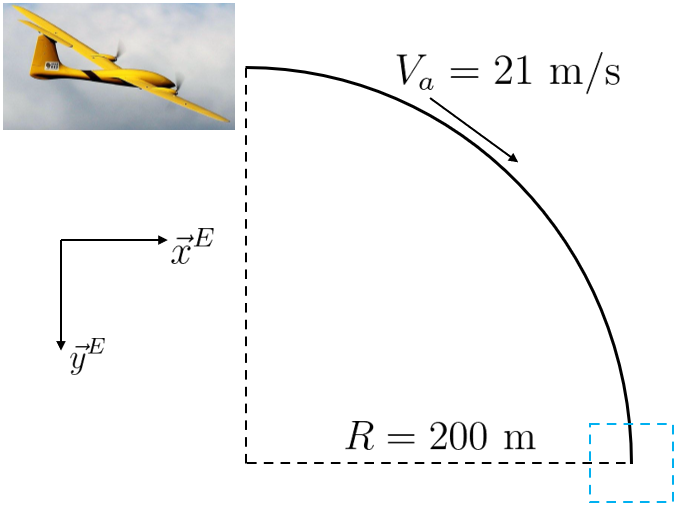
\includegraphics[scale=0.5]{turn.png}
\end{center}

You will use the aircraft \texttt{aircraftDynamics} and \texttt{lonAeroForcesAndMoments} functions developed in P3 for this assignment. If you did not complete P3, you can use the solution code posted on piazza. Template files for P4 are available by cloning the git repository at \url{https://github.com/zsunberg/Aircraft-Dynamics-Materials} and navigating to the \texttt{assignments/P4} directory. A zip file is also available at \url{https://github.com/zsunberg/Aircraft-Dynamics-Materials/raw/main/zips/assignments/P4.zip}. It is possible that there will be bugfixes to the assignment after it is released. These will be announced on Piazza.

\begin{task}
    Under the assumption that the 90 degree turn is a coordinated turn, calculate the roll angle required to complete the turn if the airspeed is 21 m/s and the turn radius is 200 m. Also, calculate the time needed to finish the turn if the turn is a perfect quarter-circle. This time, $t_{max}$, is needed in Task \ref{task:plot}. \textbf{Make sure the calculated values are printed in your \texttt{report} pdf file.}
\end{task}

\begin{task} \label{task:rollrate}
    Design a roll-rate controller (inner loop of the roll controller) of the form $\delta_a = k_a (p_c - p)$ ($J_a$ in Figure 8.26). First use the \texttt{estimateLateralSS} function to estimate the lateral state space model for the ttwistor. Then extract $\mathcal{L}_p$ and $\mathcal{L}_{\delta_a}$ from the matrix. Using the pure roll approximation, choose a gain so that the aircraft will achieve a commanded roll rate and the time constant for the roll mode is decreased by 10\% from its open-loop value.
    \textbf{Make sure the value for $k_a$ is printed in your \texttt{report} pdf file.}
\end{task}

\begin{task}
    Design a roll angle controller. \textbf{Plot the root locus} for a linear roll angle controller with the form $p_c = k_p (\phi_c - \phi)$ ($J_p$ in Figure 8.26) using the dynamics in the estimated lateral $A$ matrix and the roll-rate controller designed above. Choose a gain value that stabilizes the spiral mode and makes the spiral mode time constant near 1 second. \textbf{Plot the step response} for the roll angle controller with the desired roll angle ($\phi_c$ in Figure 18.26) as input, and the measured roll angle as output.
    \textbf{Make sure the value for $k_p$ is printed in your \texttt{report} pdf file.}
\end{task}

\begin{task} \label{task:yaw}
    Design a linear yaw damper with the form $\delta_r = -k_r r$. \textbf{Plot the root locus} for $k_r$ and choose a gain that increases the damping ratio to $0.3$ or greater and commands a rudder angle of less than $45^\circ$ for a yaw rate of $0.1$ rad/s. \textbf{Record the value of the gain $k_r$ in the designated location in the \texttt{report} pdf.}
\end{task}

\begin{task}
    Implement a roll controller and yaw damper in \texttt{controls.m} to calculate the aileron deflection $\delta_a$ and rudder deflection $\delta_r$ based on the aircraft state during the turn. 
You do not need to modify the elevator and thrust controllers that have already been implemented in the \texttt{controls} function.
\end{task}

\begin{task} \label{task:plot}
    Use the existing code under Task \ref{task:plot} of \texttt{report.m} to simulate the aircraft's motion with the nonlinear dynamics. The goal for the simulated turn is to arrive inside a box (sketched in blue in the diagram above) defined by $(x^E,y^E,z^E) = (200 \pm 5\ \text{m},200 \pm 5\ \text{m}, -1800 \pm 5 \text{m})$ after time $t_{max}$, which you calculated in Task 1. Tweak the values of the gains or the bank angle to achieve the goal.
    \textbf{In your report, include the plot produced by \texttt{plotStateHistory} plus a plot showing the path of the aircraft in the $x^E$-$y^E$ plane.}
\end{task}

\begin{task}
    Run the \texttt{evaluate} function to produce a \texttt{submission.json} file that certifies the aircraft arrives at the target with your implementation of \texttt{controls}.
\end{task}

\begin{task}
    \textbf{Optional:}
    You can add wind to the simulation with a third integer argument to the \texttt{evaluate} function. This will add a constant wind in the $y$ direction with a magnitude equal to the argument in meters per second along with gusts based on an approximation to the Dryden gust model. More information about the wind can be found in the \texttt{wind\_info.md} document in the P4 directory. Your leaderboard score will be increased by the velocity of the added wind. Note that the angle controls are limited to the interval $[-\pi/4, \pi/4]$ and the throttle is limited to $[0, 1]$. This task is completely optional and will not affect your grade.
\end{task}

\subsection*{Deliverables}
In order to use the template files, rename them by removing \texttt{TEMPLATE\_}. To produce the required report with plots, using the Matlab command \texttt{publish('report.m', 'pdf')} is highly recommended. Submit the following files to Gradescope:

\begin{itemize}[noitemsep]
    \item \texttt{submission.json} (make sure that the Gradescope autograder runs successfully when you submit!)
    \item \texttt{report.pdf} containing required output from the tasks.
    \item \texttt{controls.m}
    \item Any additional supporting functions you may have written.
\end{itemize}

\end{document}
